%-----------------------------------------------------------------------------
% header
%-----------------------------------------------------------------------------
%-----------------------------------------------------------------------------
% general document control
%\documentclass[11pt,a4paper,notitlepage]{article}
%\documentclass[journal]{ieeetr}

% journal specifics
\documentclass{article}
\usepackage{smc2012} 
\usepackage{times}
\usepackage{ifpdf}
\usepackage[english]{babel}
\usepackage{cite}
%\usepackage{mathptmx} 

% section counter
%\setcounter{secnumdepth}{1} 

% localization
\usepackage[utf8x]{inputenc}
%\usepackage[brazil]{babel}
%\usepackage{abntex}


% glossary
%\usepackage{glossaries}
%\makeglossaries
%\input{glossario}

% bibliography
%\usepackage[colorlinks,citecolor=blue,urlcolor=brown]{hyperref}
%\usepackage[alf]{abntcite}
%\usepackage[square,comma]{natbib}
%\usepackage[fixlanguage]{babelbib}
%\selectbiblanguage{portugues}


% embellishment
\usepackage{amssymb,amsmath,amsfonts}
\usepackage{booktabs}
%\numberwithin{equation}{section}
%\usepackage{enumerate}
%\usepackage[top=2.5cm, bottom=2.5cm, left=2.5cm, right=2.5cm]{geometry}
%\usepackage{xspace}
%\usepackage{colortbl}
%\usepackage{caption}
%\usepackage{mathdots}
%\usepackage{fancyhdr}
\usepackage{enumitem}
\setlist{nolistsep}


% figures
%\usepackage{graphicx}
%\usepackage{epsfig}

% math
\usepackage{amsthm}


%\usepackage{epstopdf}
%\usepackage[figure,table]{hypcap}	% corrects the hyper-anchor of figures/tables

% todo
%\usepackage[bordercolor=white,backgroundcolor=yellow!30,linecolor=black,colorinlistoftodos]{todonotes}
%\newcommand{\lembrete}[1]{\todo[color=cyan!20,inline]{\ensuremath{\rhd} #1}}


% new commands
%\newcommand{\FFT}{\texttt{FFT}\xspace}
%\newtheorem{definicao}{Definição}
%\newtheorem{exemplo}{Exemplo}
%\newtheorem{problema}{Problema}
%\newtheorem{algoritmo}{Algoritmo}
%\newtheorem{sistema}{Sistema}
\newcommand{\jclass}[1]{\texttt{\textmd{#1}}}

% hiphenation
\hyphenation{a-mount}

\usepackage{listings}
\usepackage{color}

\definecolor{dkgreen}{rgb}{0,0.4,0}
\definecolor{gray}{rgb}{0.5,0.5,0.5}
\definecolor{mauve}{rgb}{0.58,0,0.82}
\definecolor{LightCyan}{rgb}{0.7,0.9,0.9}
 
\lstset{ %
  language=C,                % the language of the code
  basicstyle=\ttfamily\footnotesize,           % the size of the fonts that are used for the code
  %numbers=left,                   % where to put the line-numbers
  numberstyle=\tiny,%\color{gray},  % the style that is used for the line-numbers
  stepnumber=1,                   % the step between two line-numbers. If it's 1, each line 
                                  % will be numbered
  numbersep=5pt,                  % how far the line-numbers are from the code
  %backgroundcolor=\color{white},      % choose the background color. You must add \usepackage{color}
  showspaces=false,               % show spaces adding particular underscores
  showstringspaces=false,         % underline spaces within strings
  showtabs=false,                 % show tabs within strings adding particular underscores
  frame=single,                   % adds a frame around the code
  %rulecolor=\color{black},        % if not set, the frame-color may be changed on line-breaks within not-black text (e.g. commens (green here))
  tabsize=2,                      % sets default tabsize to 2 spaces
  captionpos=b,                   % sets the caption-position to bottom
  breaklines=false,                % sets automatic line breaking
  breakatwhitespace=false,        % sets if automatic breaks should only happen at whitespace
  title=\lstname,                   % show the filename of files included with \lstinputlisting;
                                  % also try caption instead of title
  %keywordstyle=\color{blue},          % keyword style
  %commentstyle=\color{dkgreen},       % comment style
  %stringstyle=\color{mauve},         % string literal style
  escapeinside={\%*}{*)},            % if you want to add a comment within your code
  morekeywords={*,...},               % if you want to add more keywords to the set
  %xleftmargin=1em,
}


\newcommand{\figura}[3]{
\begin{figure}
\begin{center}
\includegraphics[width=#2\textwidth]{#1}
\caption{#3}
\label{fig:#1}
\end{center}
\end{figure}
}


%-----------------------------------------------------------------------------
% journal specific commands
%-----------------------------------------------------------------------------

%user defined variables
\def\papertitle{Real time digital audio processing using Arduino}
\def\firstauthor{André Jucovsky Bianchi}
\def\secondauthor{Marcelo Queiroz}
\def\thirdauthor{Third author}

%-----------------------------------------------------------------------------
% Dados do trabalho
%\title{}
%\author{André Jucovsky Bianchi \\
%\small{Departamento de Ciência da Computação \\
%Instituto de Matemática e Estatística \\
%Universidade de São Paulo \\
%\texttt{ajb@ime.usp.br}}}

\newif\ifpdf
\ifx\pdfoutput\relax
\else
   \ifcase\pdfoutput
      \pdffalse
   \else
      \pdftrue
\fi

\ifpdf % compiling with pdflatex
  \usepackage[pdftex,
    pdftitle={\papertitle},
    pdfauthor={\firstauthor, \secondauthor, \thirdauthor},
    bookmarksnumbered, % use section numbers with bookmarks
    pdfstartview=XYZ % start with zoom=100% instead of full screen; 
                     % especially useful if working with a big screen :-)
   ]{hyperref}
  %\pdfcompresslevel=9

  \usepackage[pdftex]{graphicx}
  % declare the path(s) where your graphic files are and their extensions so 
  %you won't have to specify these with every instance of \includegraphics
  \graphicspath{{./img/}}
  \DeclareGraphicsExtensions{.pdf,.jpeg,.png}

  \usepackage[figure,table]{hypcap}

  \usepackage{epstopdf}

\else % compiling with latex
  \usepackage[dvips,
    bookmarksnumbered, % use section numbers with bookmarks
    pdfstartview=XYZ % start with zoom=100% instead of full screen
  ]{hyperref}  % hyperrefs are active in the pdf file after conversion

  \usepackage[dvips]{epsfig,graphicx}
  % declare the path(s) where your graphic files are and their extensions so 
  %you won't have to specify these with every instance of \includegraphics
  \graphicspath{{./img/}}
  \DeclareGraphicsExtensions{.eps}

  \usepackage[figure,table]{hypcap}
\fi

%setup the hyperref package - make the links black without a surrounding frame
\hypersetup{
    colorlinks,%
    citecolor=black,%
    filecolor=black,%
    linkcolor=black,%
    urlcolor=black
}

% Title.
% ------
\title{\papertitle}

% Authors
% Please note that submissions are NOT anonymous, therefore 
% authors' names have to be VISIBLE in your manuscript. 
%
% Single address
% To use with only one author or several with the same address
% ---------------
%\oneauthor
%   {\firstauthor} {Affiliation1 \\ %
%     {\tt \href{mailto:author1@smcnetwork.org}{author1@smcnetwork.org}}}

%Two addresses
%--------------
\twoauthors
  {\firstauthor} {Computer Science Department \\
                  University of São Paulo \\ %
    {\tt \href{mailto:ajb@ime.usp.br}{ajb@ime.usp.br}}}
  {\secondauthor} {Computer Science Department \\
                  University of São Paulo \\ %
    {\tt \href{mailto:mqz@ime.usp.br}{mqz@ime.usp.br}}}

% Three addresses
% --------------
% \threeauthors
%   {\firstauthor} {Affiliation1 \\ %
%     {\tt \href{mailto:author1@smcnetwork.org}{author1@smcnetwork.org}}}
%   {\secondauthor} {Affiliation2 \\ %
%     {\tt \href{mailto:author2@smcnetwork.org}{author2@smcnetwork.org}}}
%   {\thirdauthor} { Affiliation3 \\ %
%     {\tt \href{mailto:author3@smcnetwork.org}{author3@smcnetwork.org}}}

%-----------------------------------------------------------------------------
% Document
\begin{document}

%
\capstartfalse
\maketitle
\capstarttrue

%
% sumário
%\tableofcontents

\maketitle

\begin{abstract}

% contexto do trabalho
% problema que resolve
% por que é um problema interessante
% quais as consequências

In the search for low-cost, highly available devices for real time audio
processing for scientific or artistic purposes, the Arduino platform comes in
as a handy alternative as a chordless, versatile audio processor. Despite the
fact that Arduinos are generally used for controlling and interfacing with
other devices, its builtin ADC/DAC allows for capturing and emitting raw audio
signals with very specific constraints. In this work we dive into the
microcontroller's structure to understand what can be done and what are the
limits of the platform when working with real time digital signal processing.
We evaluate the behaviour of some common DSP algorithms and expose limitations
and possibilities of using the platform in this context.


\end{abstract}

%-----------------------------------------------------------------------------
%  ___       _                 _            _   _             
% |_ _|_ __ | |_ _ __ ___   __| |_   _  ___| |_(_) ___  _ __  
%  | || '_ \| __| '__/ _ \ / _` | | | |/ __| __| |/ _ \| '_ \ 
%  | || | | | |_| | | (_) | (_| | |_| | (__| |_| | (_) | | | |
% |___|_| |_|\__|_|  \___/ \__,_|\__,_|\___|\__|_|\___/|_| |_|
%-----------------------------------------------------------------------------

\section{Introduction}


Arduino is the name of a hardware and software project started in 2005 which
aims to simplify the interface of electric-electronic devices with a
microcontroller. It evolved from the Processing software IDE (2001) and the
Wiring software and hardware prototyping platform (2003). Hardware, software
and documentation designs are published under free licenses (Creative Commons
BY-SA 2.5, GPL/LGPL and CC BY-SA 3.0 respectively) and a large community has
grown to provide code and support for newcomers. Nowadays, many Arduino
hardware designs are available and range from more limited 8-bit
microcontrollers to fully featured 32-bit ARM CPUs. Among these, other
Arduino's advantages for academic and artistic use are its mobility (because
of its low power needs and possibility of running on batteries for hours, if
not days depending on the use), expandability (because of its standardized
interface for attaching so called hardware \emph{shields}) and price (selling
for under 20 US dollars online).

Despite all these advantages, the platform has a somewhat limited processing
power when compared to standard processors available in the market for
specific or general uses. In this work, we aim to systematically expose the
platform's possibilities for carrying real time digital audio processing tasks
so there can be more accurate elements to be taken into account when making
the choice for a platform.


\subsection{Related work}




\subsection{Text organization}


%-----------------------------------------------------------------------------
% __  __      _   _               _     
%|  \/  | ___| |_| |__   ___   __| |___ 
%| |\/| |/ _ \ __| '_ \ / _ \ / _` / __|
%| |  | |  __/ |_| | | | (_) | (_| \__ \
%|_|  |_|\___|\__|_| |_|\___/ \__,_|___/
%-----------------------------------------------------------------------------

\section{Methods}
\label{sec:methods}

In order to meet the needs for real time audio processing, the microcontroller
has to be tweaked so we can capture, process and output analog audio. Each of
these tasks can be performed in a variety of ways, and for this examination we
chose to go with the basic functionalities of the platform.

In this investigation, we used an Arduino Duemilanove with an ATmega328P
microcontroller, a very modest version of the platform. It has an 8-bit RISC
central processor, operates with a base frequency of 16~MHz, and has memory
capacity of 32~KB for program storage and 2~KB for random access.

\subsection{Microcontroller's elements}

\setlength{\itemsep}{0em}

To be able to know how to configure the platform to suit our needs, a general
understanding of the inner workings of a microcontroller is needed. The Atmel
Atmel megaAVR series microcontroller is comprised of several components, some
of which are fundamental for our investigation and so will be briefly covered
in this section.

\subsubsection{Clocks}

Clocks provide the frequencies in which the different parts of the
microcontroller work. They are basically either emitters or dividers of square
wave signals that provide the frequency of operation of the CPU, the ADC,
the memory access, etc. Possible sources of clock frequencies are crystal
and RC oscillators.

A useful concept associated with clocks is the one of a \emph{prescaler}.
Prescalers are dividers for clock frequencies that either actually lower the
frequency of a clock or at least trigger specific interrupts on a power of two
fraction of a clock's frequency.

The \emph{system clock} provides the system's base frequency of operation. In
our study, we make use of the system clock prescaler to control the PWM
frequency that drives our DSP mechanism, as we will see in the section
\ref{sec:pwm}. Another important clock is the \emph{I/O clock} used for
feeding a frequency to most of the input/output mechanisms.

\subsubsection{Registers and interrupts}

The microcontroller's CPU is comprised of an arithmetic logic unit that works
with 32 \emph{registers} -- portions of memory that provide data for
computation as well as determine the execution flow of the program. An
\emph{interrupt} is a deviation from the execution flow that can be triggered
by a variety of events in the system, usually by setting values on specific
registers.

In our case, interrupts are of extreme value as they are the low level
structures that allow us to execute code with a somewhat fixed frequency (at
least if we assume that the clock frequency is fixed in relation with real
time).

\subsubsection{Timers/counters}

A \emph{timer}, or \emph{counter}, is a register whose value is automatically
incremented according to a specific clock. A certain timer has a fixed length
in bits and may have lots of interrupts associated with its behaviour. When a
counter hits its maximum value, for example, it is reset to zero and signals
an overflow interrupt, which may cause a function to be called.

Timers are important in the context of DSP because they provide the way to
perform many of the DSP chain tasks, as for example to periodically launch the
sampling function (that fills the input buffer) and to emmit a PWM square wave
which after (analog) filtering causes the digital signal to be converted back
to analog. The ATmega328P has two bit counters and one 16 bit counter, each
having different sets of features but all being capable of doing PWM.

\subsubsection{Input and output pins}

Microcontrollers can receive and emit digital signal through \emph{I/O pins},
which in the case of the the Arduino board are conveniently mounted in a way
it is easy to plug other components and boards. These pins are read from and
written to according to frequencies governed by different clocks (I/O, ADC and
others).

In principle, the microcontroller pins are designed to work with binary
signals represented by two different voltages, in general 0~V and 5~V, having
a threshold value to account for small deviations from these reference
voltages. Despite that, I/O pins come equipped with handy mechanisms for
sampling input signals with voltage varying between the reference extremes,
and also to generate waveforms that can be filtered to approximate varying
output signals of the same nature. These mechanisms are, respectively, the
analog-to-digital converter (ADC) and the pulse-width modulation (PWM), which
will be seen in the next couple of sessions.


\subsubsection{Memory}

The microcontroler has 3 different memory spaces: 32~KB of persistent flash memory for
program storage, 2~KB of non-persistent SRAM memory for data storage and 1~KB
of persistent EEPROM memory for data storage. The following table summarizes
some differences between each type of memory:

\begin{center}
\begin{tabular}{crrr}
\toprule
\toprule
\multicolumn{1}{c}{\footnotesize{type}} &
\multicolumn{1}{c}{\footnotesize{size (KB)}} &
\footnotesize{\parbox{5em}{write time (clock ticks)}} &
\footnotesize{\parbox{5em}{endurance (write/erase cycles)}} \\
\midrule
Flash  & 32 & 1 & 10,000 \\
SRAM   & 2  & 2 & 10,000 \\
EEPROM & 1  & 30 & 100,000 \\ 
\bottomrule
\end{tabular}
\end{center}



\subsection{Audio in: ADC}

Data can flow into the microcontroller in a variety of ways, the most basic
being an embedded serial communication mechanism and the input pins. The
former mechanism can feed digital data directly to memory, while the latter
can either read 1 bit (as explained in the last section) or sample an
intermediate value between the reference voltages using 8 or 10 bits for
representing that value.

Rather than providing the microcontroller with digital data, our setup uses
the analog-to-digital conversion to sample an audio signal using the
microcontroller pins' ADC mechanism. This choice was made so the signal can be
directly connected to the microcontroller (i.e. no external device has to be
used for sampling) and we can study the device's performance taking into
account this crucial step in the digital audio processing chain.

The ADC uses a \emph{Sample and Hold} circuit that holds the input voltage
at a constant level until the end of the conversion. This fixed voltage is
then successively compared with reference voltages to obtain a 10 bit
approximation. If a faster conversion is desired, precision can be sacrificed
and the first 8 bits can be read before the last 2 are computed. Conversion
time takes between 13 and 250~$\mu$s, depending on several configuration
parameters given to the ADC mechanism.

As noted before, the ADC mechanism has a dedicated clock to ensure conversion
can occur independently of other microcontroller parts. Also, the mechanism
can be triggered manually (on demand) or automatically (a new conversion
starts as soon as the last one finishes).

\subsection{Audio out: PWM}
\label{sec:pwm}

Once the input signal has been sampled and processed, one way to convert
it back to analog is to use the embedded PWM mechanism that is available in
some of the output pins of the microcontroller. PWM is a technique for
representing an intermediate value from two reference values that can have its
output filtered to reconstruct a bandwidth limited signal. In our case, this
filtering is made from a simple RC circuit that stands between the output pin
and a normal speaker.

For outputting the result, PWM conversion is used, followed by a simple
low pass filter.

PWM characteristics:

\begin{itemize}
    \item 6 output channels.
    \item Different modes of operation (fast PWM and phase correct PWM).
    \item prescaler.
    \item Two 8-bit counters and one 16-bit counter.
    \item Overflow interrupt.
\end{itemize}

\figura{pwmmeu}{0.40}{TODO: change captions.}
%\figura{pwm2}{0.35}{TODO: change captions.}
\figura{Pwm}{0.45}{TODO: change captions.}

Explain how we use PWM interrupts to determine the frequency of operation of
our DSP system (and other possibilities of how this could be done).


\subsection{Processing}

The main constraint in real time DSP is, of course, the amount of time
available for the computation of output samples: they must be ready to be
consumed by the playback hardware or else glitches and other unwanted
artifacts will possibly be introduced in the signal. One round of sample
analysis, processing and calculation of a new sample is called a \emph{DSP
cycle}. Many algorithms, though, operate in blocks of samples, consuming and
producing a whole block of samples in each round. Naturally, in these cases
the period of the DSP cycle is the period of one sample times the size of the
DSP block. If the DSP block period is of $N$ samples and the sample rate is
$R$~Hz, then the DSP cycle period is given by $T_{DSP}=\frac{N}{R}$ seconds.

In order to implement this behaviour in the microcontroller, we have to find a
way to (1) accumulate input samples in a buffer, (2) schedule a periodic call
to a function that will process the samples in this buffer, and (3) output
modified samples in a timely fashion. One possible solution is to use a
timer's overflow interrupt.

\subsubsection{DSP cycles}

\begin{itemize}
    \item We need a mechanism to periodically call a function that will work
    on a block of samples.
\end{itemize}

\subsubsection{ADC conversion}

The table below shows a measurement of conversion time using different
prescaler values for the ADC clock:

\begin{center}
\begin{tabular}{crrrr}
\toprule
\toprule
\footnotesize{prescaler} & \footnotesize{$f_\text{ADC}$ (KHz)} &
\footnotesize{$T_\text{ADC}$ ($\mu$s)} & \footnotesize{$\tilde{T}_\text{conv}$ ($\mu$s)} & \footnotesize{$\tilde{f}_\text{conv}$ ($\approx$Hz)} \\
\midrule
2 & 8.000 & 0,125 & 12,61 & 79.302\\
4 & 4.000 & 0,25 & 16,06  & 62.266 \\
%\rowcolor{grey}
8 & 2.000 & 0,50 & 19,76  & 50.607 \\
16& 1.000 & 1 & 20,52  & 48.732 \\
32& 500 & 2 & 34,80  & 28.735 \\
64& 250 & 3 & 67,89  & 14.729 \\
128& 125 & 8 & 114,85 & 8.707  \\
\bottomrule
\end{tabular}
\end{center}

These measurements were made using the \texttt{micros()} function of the
Arduino library API, which has a resolution of about 4~$\mu$s.

Obs:
\begin{itemize}
  \item The resolution of the \texttt{micros()} function is of 4~$\mu$s.
  \item Conversion period $\approx$ $14.5 \times T_\text{ADC}$. 
  \item $R=44100$~Hz $\Rightarrow$ $T_\text{amostra} \approx 22.67~\mu$s.
  \item $R=31250$~Hz $\Rightarrow$ $T_\text{amostra} = 32.00~\mu$s.
\end{itemize}

ADC parameter choice:

\begin{itemize}
    \item Left-aligned conversion (8 bits).
    \item Prescaler equals to 8.
\end{itemize}

\subsubsection{PWM}

Frequency of operation given an 8-bit counter and different values for
prescaler:

\begin{center}
\begin{tabular}{crrrr}
\toprule
\toprule
\footnotesize{prescaler} &
\footnotesize{$f_\text{incr}$ (KHz)} &
\footnotesize{$f_\text{overflow}$ (Hz)}  \\
\midrule
1 & 16.000 & 62.500 \\
8 & 2.000 & 7.812 \\
32 & 500 & 1.953 \\
64 & 250 & 976 \\
128 & 125 & 488 \\
256 & 62,5 & 244 \\
1024 & 15,625 & 61 \\
\bottomrule
\end{tabular}
\end{center}

Chose parameters:

\begin{itemize}
  \item \emph{Fast PWM}.
  \item 8-bit counter.
  \item Prescaler value of 1.
  \item Overflow frequency: 16~MHz / 1 / $2^8$ = 62500~Hz.
  \item Sample generation frequency: 31250~Hz.
\end{itemize}

\subsubsection{Putting it all together}

\begin{lstlisting}
/* 1. read from ADC input */
x[ind] = ADCH;

/* 2. write to PWM output */
OCR2A = y[(ind-MIN_DELAY)&(BUFFER_SIZE-1)];

// 3. signal availability of new sample block
if ((ind & (BLOCK_SIZE - 1)) == 0) {
  rind = (ind-BLOCK_SIZE) & (BUFFER_SIZE-1);
  dsp_block = true;
}

/* 4. increment read/write buffer index */
ind++;
ind &= BUFFER_SIZE - 1;

/* 5. start new ADC conversion */
sbi(ADCSRA,ADSC); 
\end{lstlisting}



\subsection{Benchmarking}

Once we have a way to input and output analog audio signals to and from the
Arduino board, then we can start to experiment and measure the time it takes
to perform common DSP routines in this environment.

Some questions arise immediately from such a constraint:

\begin{itemize}
    \item What is the maximum amount of operations that can be carried in real
    time?
    \item Which implementation details make a difference?
    \item What is the quality of the resulting audio signal?
\end{itemize}

\subsubsection{Additive synthesis}

An additive synthesis is the process of constructing a more complex waveform
by adding together several more basic waveforms (see Figure \ref{fig:add}).
This technique has been widely used for synthesizing new sounds as well as
resynthesizing signals after they went through some computational procedure.

\figura{add}{0.20}{Additive synthesis.}


The high level code for a simple additive synthesis can be seen below:

\begin{lstlisting}[caption=Additive synthesis algorithm.]
for (n = 0; n < N; n++)
{
  angle = 2.0 * M_PI * t;
  y[n] = 0.0;
  for (k = 0; k < numFreqs; k++)
    y[n] += r[k]*sin(f[k] * angle);
  t += 1.0 / SR;
}
\end{lstlisting}

\subsubsection{Time-domain convolution}

Frequency-domain multiplication of spectra correspond to time-domain
convolution of signals, and such an operation allows for frequency filtering.
The time-domain implementation of convolution is a widely used technique in
many computer music algorithms and the general scheme can be seen in Figure
\ref{fig:FIR_Filter}.

\figura{FIR_Filter}{0.35}{TODO: change caption}

The high-level code for a time-domain convolution is:

\begin{lstlisting}
for (k = 0; k < N; k++)
  y[n] += b[k]*x[n-k];
\end{lstlisting}

\subsubsection{Fast Fourier Transform}

The Fast Fourier Transform (FFT) is a clever implementation of the traditional
Fourier Transform that brings its complexity down from $O(n^2)$ to
$O(n\log(n))$, where $n$ is the number of time-domain digital samples or,
equivalently, the number of frequency bins that describe the frequency
spectrum of the signal after the Transform computation. The FFT algorithm
takes advantage of redundancy and symmetry on intermediary steps of the
calculation and is used in many signal processing algorithms (see Figure
\ref{fig:butterfft}).

%-----------------------------------------------------------------------------
%\figura{./img/fft1.pdf}{0.35}{TODO: change caption}


\figura{butterfft}{0.35}{The FFT uses a divide-and-conquer approach and saves
intermediate results to accelerate the calculation of a signal spectrum. The
figure shows one step of an 8-point FFT calculation and how the results map to
frequency bins.}
%-----------------------------------------------------------------------------

\subsubsection{Benchmarking}

Each of the algorithms mentioned in the last sections have different
computational costs in terms of number of integer and floating-point
operations, and quantity of memory reads and writes (and amount of memory
accessed in each of these operations). 

In the context of real time audio processing in the Arduino, the algorithms mentioned above
bring natural questions regarding feasibility of processing:

\begin{itemize}
  \item Additive synthesis: what is the maximum number of oscillators that can
  be used to compute a new waveform in real time?
  \item Time-domain convolution: what is the maximum length of a filter that
  can be applied to an audio signal in real time?
  \item FFT: what is the maximum length of an FFT that can be computed in real time?
\end{itemize}


\section{Análise de desempenho}

%-----------------------------------------------------------------------------
\begin{frame}[fragile]{Desempenho para processamento em tempo real}
Perguntas:
\begin{itemize}
  \item Qual é número máximo de operações computáveis em tempo real?
  \item Quais detalhes de implementação fazem diferença?
  \item Qual é a qualidade do áudio resultante?
\end{itemize}
\vspace{2em}
Implementações:
\begin{itemize}
  \item Síntese aditiva.
  \item Convolução no domínio do tempo.
  \item FFT.
\end{itemize}
\end{frame}
%-----------------------------------------------------------------------------

%-----------------------------------------------------------------------------
%     _       _     _ _ _   _             ____              _   _     
%    / \   __| | __| (_) |_(_)_   _____  / ___| _   _ _ __ | |_| |__  
%   / _ \ / _` |/ _` | | __| \ \ / / _ \ \___ \| | | | '_ \| __| '_ \ 
%  / ___ \ (_| | (_| | | |_| |\ V /  __/  ___) | |_| | | | | |_| | | |
% /_/   \_\__,_|\__,_|_|\__|_| \_/ \___| |____/ \__, |_| |_|\__|_| |_|
%                                               |___/
%-----------------------------------------------------------------------------

\subsection{Síntese Aditiva}

%-----------------------------------------------------------------------------
\begin{frame}{Síntese aditiva}
\begin{figure}
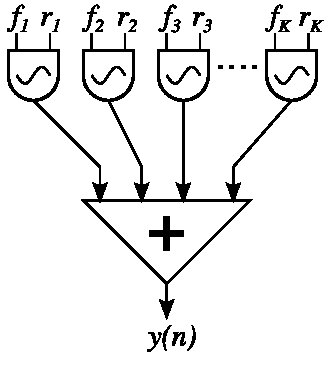
\includegraphics[height=0.8\textheight]{./img/add.pdf}
\end{figure}
\end{frame}
%-----------------------------------------------------------------------------

%-----------------------------------------------------------------------------
\begin{frame}[fragile]{Síntese aditiva}
\noindent Código em alto nível:
\begin{lstlisting}
for (n = 0; n < N; n++)
{
  angle = 2.0 * M_PI * t;
  y[n] = 0.0;
  for (k = 0; k < numFreqs; k++)
    y[n] += r[k]*sin(f[k] * angle);
  t += 1.0 / SR;
}
\end{lstlisting}
Implementação da linha 6:
\begin{lstlisting}
  ind[k] = (ind[k]+f[k]) & (SINETABLE_SIZE-1);
  y[n&(BUFFER_SIZE-1)] += sine[ind[k]] >> pad;
\end{lstlisting}
\end{frame}
%-----------------------------------------------------------------------------


%-----------------------------------------------------------------------------
\begin{frame}{Síntese aditiva}{Tipo e número de operações fazem a diferença}
%\begin{itemize}
%  \item Taxa de amostragem: $R = 31.250$~Hz (freq. até 15.625~Hz).
%  \item Tamanhos de bloco: 128 amostras.
%  \item Período do ciclo DSP: $T=\frac{N}{R}=4,096$~ms.
%\end{itemize}
\begin{figure}
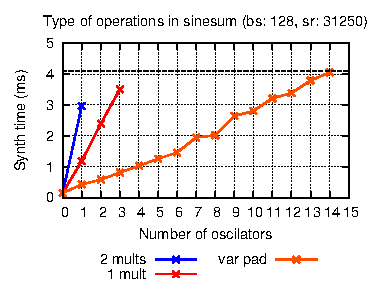
\includegraphics[width=0.8\textwidth]{./img/operations-128-31250.pdf}
\end{figure}
\end{frame}
%-----------------------------------------------------------------------------

%-----------------------------------------------------------------------------
\begin{frame}{Síntese aditiva}{Resultados para blocos de diferentes tamanhos}
%\begin{itemize}
%  \item Taxa de amostragem: $R = 31.250$~Hz (freq. até 15.625~Hz).
%  \item Tamanhos de bloco: 32, 64 e 128 amostras.
%  \item Período do ciclo DSP: $T=\frac{N}{R}$.
%\end{itemize}
\begin{figure}
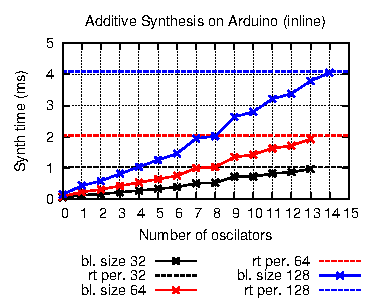
\includegraphics[width=0.8\textwidth]{./img/sinesum-comparison.pdf}
\end{figure}
\end{frame}
%-----------------------------------------------------------------------------

%-----------------------------------------------------------------------------
\begin{frame}{Síntese aditiva}{Resultados para blocos de diferentes tamanhos}
%\begin{itemize}
%  \item Taxa de amostragem: $R = 31.250$~Hz (freq. até 15.625~Hz).
%  \item Tamanhos de bloco: 32, 64 e 128 amostras.
%  \item Período do ciclo DSP: $T=\frac{N}{R}$.
%\end{itemize}
\begin{figure}
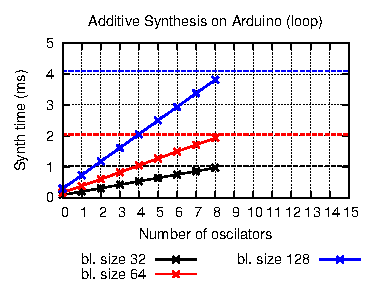
\includegraphics[width=0.8\textwidth]{./img/sinesum-comparison-for.pdf}
\end{figure}
\end{frame}
%-----------------------------------------------------------------------------


%-----------------------------------------------------------------------------
\begin{frame}{Síntese aditiva}{Resultados para diferentes taxas de amostragem}
%\begin{itemize}
%  \item Taxas de amostragem: $R_1 = 31.250$~Hz e $R_2=15.625$~Hz.
%  \item Tamanhos de bloco: 128 amostras.
%  \item Período do ciclo DSP: $T=\frac{N}{R}=8,192$~ms.
%\end{itemize}
\begin{figure}
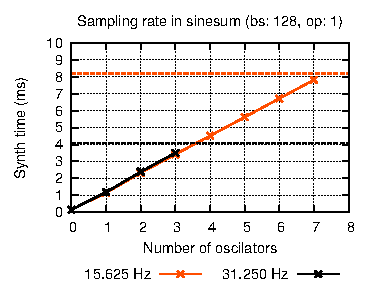
\includegraphics[width=0.8\textwidth]{./img/frequencies-128-1.pdf}
\end{figure}
\end{frame}
%-----------------------------------------------------------------------------

%-----------------------------------------------------------------------------
\begin{frame}{Síntese aditiva}{Resumo dos resultados}
Número de osciladores máximo em cada cenário ($R=31.250$~Hz):
\begin{center}
\begin{tabular}{rcccc}
\toprule
\toprule
block size  & 2op & 1op & pad+for & pad \\
\midrule
32  & 2 & 4 & 8 & 14 \\
64  & 2 & 4 & 8 & 14 \\
128 & 2 & 4 & 8 & 15 \\
\bottomrule
\end{tabular}
\pause
\end{center}
\begin{itemize}
  \item Exemplo: soma de harmônicos de 200~Hz.
\end{itemize}
\end{frame}
%-----------------------------------------------------------------------------


%-----------------------------------------------------------------------------
%   ____                      _       _   _             
%  / ___|___  _ ____   _____ | |_   _| |_(_) ___  _ __  
% | |   / _ \| '_ \ \ / / _ \| | | | | __| |/ _ \| '_ \ 
% | |__| (_) | | | \ V / (_) | | |_| | |_| | (_) | | | |
%  \____\___/|_| |_|\_/ \___/|_|\__,_|\__|_|\___/|_| |_|
%                                                       
%-----------------------------------------------------------------------------

\subsection{Convolução no domínio do tempo}

%-----------------------------------------------------------------------------
\begin{frame}{Convolução no domínio do tempo}
\begin{figure}
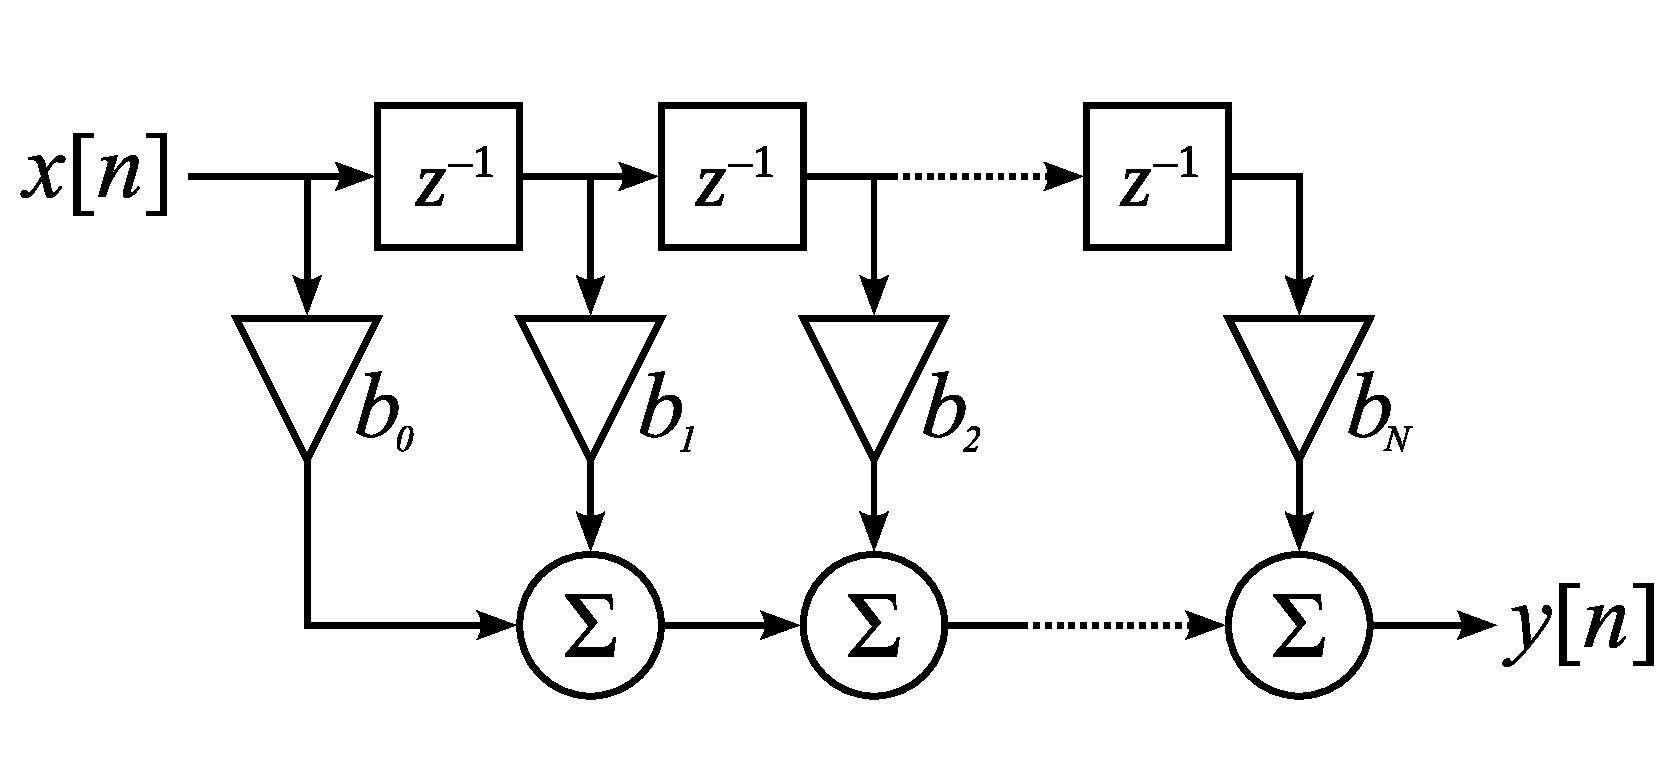
\includegraphics[width=\textwidth]{./img/FIR_Filter.pdf}
\end{figure}
\end{frame}
%-----------------------------------------------------------------------------

%-----------------------------------------------------------------------------
\begin{frame}[fragile]{Convolução no domínio do tempo}
{Qual o tamanho máximo de um filtro computável em tempo real?}
Código em alto nível:
\begin{lstlisting}
for (k = 0; k < N; k++)
  y[n] += b[k]*x[n-k];
\end{lstlisting}
Implementação:
\begin{lstlisting}
for (int n = 0; n < N; n++) {
  int yn = 0, xtmp;
  for (int i = 0; i < order; i++) {
    xtmp = 127 - TMOD(x, n-i, BUFFER_SIZE);
    yn += xtmp * 10 / 100;
  }
  LIMIT(yn); /* limita a +- 127 */
  TMOD(y, n, BUFFER_SIZE) = 127 + yn;
}
\end{lstlisting}
\end{frame}
%-----------------------------------------------------------------------------

%-----------------------------------------------------------------------------
\begin{frame}{Convolução no domínio do tempo}{Resultados para blocos de diferentes tamanhos}
%\begin{itemize}
%  \item Taxa de amostragem: $R = 31.250~Hz$.
%  \item Tamanhos de bloco: 32, 64, 128 e 256 amostras.
%  \item Tipo de operação: pad constante.
%\end{itemize}
\begin{figure}
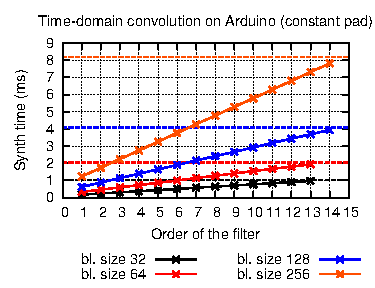
\includegraphics[width=0.8\textwidth]{./img/convolution-comparison-cpad.pdf}
\end{figure}
\end{frame}
%-----------------------------------------------------------------------------


%-----------------------------------------------------------------------------
\begin{frame}{Convolução no domínio do tempo}{Resultados para blocos de diferentes tamanhos}
%\begin{itemize}
%  \item Taxa de amostragem: $R = 31.250~Hz$.
%  \item Tamanhos de bloco: 32, 64, 128 e 256 amostras.
%  \item Tipo de operação: pad variável.
%\end{itemize}
\begin{figure}
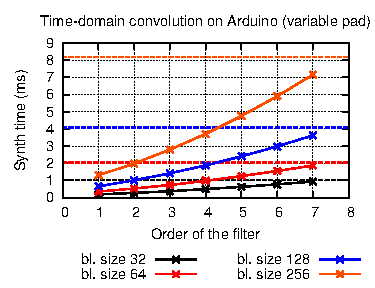
\includegraphics[width=0.8\textwidth]{./img/convolution-comparison-vpad.pdf}
\end{figure}
\end{frame}
%-----------------------------------------------------------------------------


%-----------------------------------------------------------------------------
\begin{frame}{Convolução no domínio do tempo}{Resultados para blocos de diferentes tamanhos}
%\begin{itemize}
%  \item Taxa de amostragem: $R = 31.250~Hz$.
%  \item Tamanhos de bloco: 32, 64, 128 e 256 amostras.
%  \item Tipo de operação: multiplicação.
%\end{itemize}
\begin{figure}
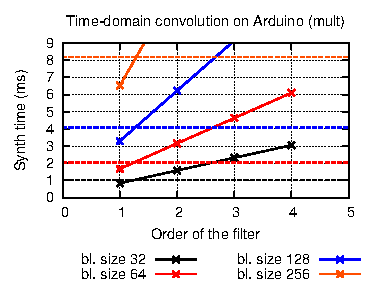
\includegraphics[width=0.8\textwidth]{./img/convolution-comparison-mult.pdf}
\end{figure}
\end{frame}
%-----------------------------------------------------------------------------

%-----------------------------------------------------------------------------
\begin{frame}{Convolução no domínio do tempo}{Resultados para blocos de diferentes tamanhos}
Ordem máxima do filtro FIR em cada cenário ($R=31.250$~Hz):
\begin{center}
\begin{tabular}{rccc}
\toprule
\toprule
\footnotesize{block size}  & \footnotesize{multiplicação} & \footnotesize{pad variável} & \footnotesize{pad constante} \\
\midrule
32  & 1 & 7 & 13 \\
64  & 1 & 7 & 13 \\
128 & 1 & 7 & 14 \\
256 & 1 & 7 & 14 \\
\bottomrule
\end{tabular}
\end{center}
\end{frame}
%-----------------------------------------------------------------------------

%-----------------------------------------------------------------------------
\begin{frame}{Convolução no domínio do tempo}{Exemplo: moving average}
%\begin{itemize}
%  \item Taxa de amostragem: $R = 31.250~Hz$.
%  \item Tamanhos de bloco: 32, 64, 128 e 256 amostras.
%  \item Tipo de operação: pad variável.
%\end{itemize}
\begin{figure}
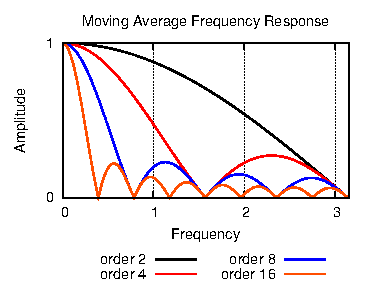
\includegraphics[width=0.8\textwidth]{./img/moving.pdf}
\end{figure}
\end{frame}
%-----------------------------------------------------------------------------

%-----------------------------------------------------------------------------
%  _____ _____ _____ 
% |  ___|  ___|_   _|
% | |_  | |_    | |  
% |  _| |  _|   | |  
% |_|   |_|     |_|  
%
%-----------------------------------------------------------------------------
\subsection{FFT}

%-----------------------------------------------------------------------------
\begin{frame}{Fast Fourier Transform}
\begin{figure}
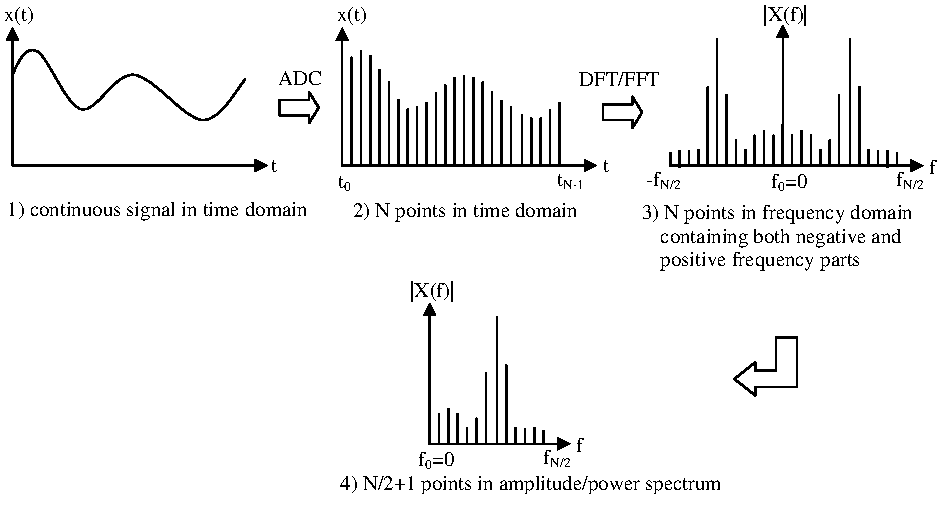
\includegraphics[width=\textwidth]{./img/fft1.pdf}
\end{figure}
\end{frame}
%-----------------------------------------------------------------------------

%-----------------------------------------------------------------------------
\begin{frame}{Fast Fourier Transform}
A transformada discreta de Fourier (DFT) de um vetor de $N$ pontos é:
\[
X_k = \sum_{n=0}^{N-1} x_n e^{-i 2 \pi k \frac{n}{N}}, \hspace{2em} k = 1, \dots, N-1.
\]
\begin{itemize}
  \item Implementação ingênua da DFT: $O(N^2)$.
  \item Implementações de FFT para diferentes valores de N: $O(N \log(N))$.
\end{itemize}
\end{frame}
%-----------------------------------------------------------------------------

%-----------------------------------------------------------------------------
\begin{frame}{Fast Fourier Transform}
\begin{figure}
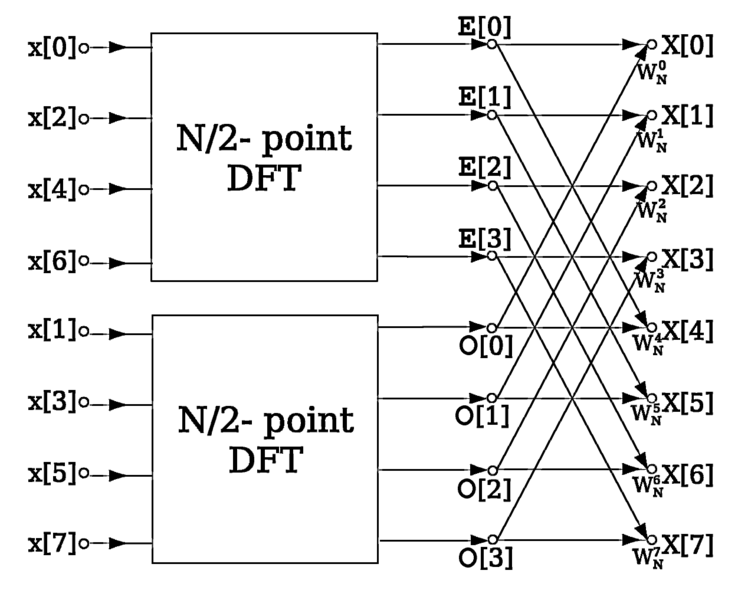
\includegraphics[height=0.8\textheight]{./img/butterfft.png}
\end{figure}
\end{frame}
%-----------------------------------------------------------------------------


%-----------------------------------------------------------------------------
%\begin{frame}{Fast Fourier Transform}
%Algoritmo de Cooley-Tukey para vetores de tamanho $2^k=2m$:
%\[
%  \begin{matrix} X_k & =
%& \sum \limits_{m=0}^{N/2-1} x_{2m}     e^{-\frac{2\pi i}{N} (2m)k}   +
%  \sum \limits_{m=0}^{N/2-1} x_{2m+1} e^{-\frac{2\pi i}{N} (2m+1)k}.
%  \end{matrix}
%\]
%Chamando de $E_k$ (e respectivamente $O_k$) o vetor de tamanho 2m com os
%índices pares (ímpares) $x_{2m}$ ($x_{2m+1}$), teremos:
%\[
%\begin{matrix} X_k & =
%& \left\{
%\begin{matrix}
%E_k + e^{-\frac{2\pi i}{N}k} O_k & \mbox{if } k < N/2 \\ \\
%E_{k-N/2} - e^{-\frac{2\pi i}{N} (k-N/2)} O_{k-N/2} & \mbox{if }
%k \geq N/2. \end{matrix} \right. \end{matrix}
%\]
%\end{frame}
%-----------------------------------------------------------------------------

%-----------------------------------------------------------------------------
\begin{frame}[fragile]{Fast Fourier Transform}
Código em altíssimo nível:
\begin{lstlisting}
four1(x, N, 1); /* O(N*log(N)) */
\end{lstlisting}
\begin{itemize}
  \item Qual é o tamanho máximo de uma FFT computável em tempo real?
\end{itemize}
\end{frame}
%-----------------------------------------------------------------------------


%-----------------------------------------------------------------------------
\begin{frame}{Fast Fourier Transform}{Resultados}
\begin{figure}
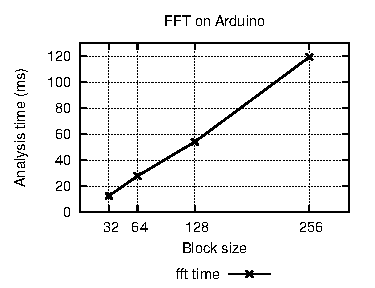
\includegraphics[width=0.8\textwidth]{./img/fft.pdf}
\end{figure}
\end{frame}
%-----------------------------------------------------------------------------

%-----------------------------------------------------------------------------
\begin{frame}{Fast Fourier Transform}{Resultados}
Determinação de frequência máxima:
\begin{itemize}
  \item Média de 428,15~$\mu$s por amostra.
  \item Frequência máxima $\approx$ 2.335~Hz.
  \item Pré-escalonador PWM de 32 $\Rightarrow$ $R=1.953$~Hz.
\end{itemize}
\end{frame}
%-----------------------------------------------------------------------------

%-----------------------------------------------------------------------------
\begin{frame}{Fast Fourier Transform}{Resultados}
\begin{figure}
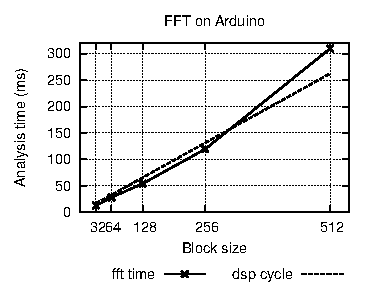
\includegraphics[width=0.8\textwidth]{./img/fft2.pdf}
\end{figure}
\end{frame}
%-----------------------------------------------------------------------------


%-----------------------------------------------------------------------------
% ____  _                        _             
%|  _ \(_)___  ___ _   _ ___ ___(_) ___  _ __  
%| | | | / __|/ __| | | / __/ __| |/ _ \| '_ \ 
%| |_| | \__ \ (__| |_| \__ \__ \ | (_) | | | |
%|____/|_|___/\___|\__,_|___/___/_|\___/|_| |_|
%-----------------------------------------------------------------------------

\section{Discussion}
\label{sec:discussion}

From the results of our experiments, it is obvious that implementation details
make a big difference in the amount of computation. 

\begin{itemize}
    \item The types used (byte, unsigned long, int, float, etc) are
    fundamental.
    \item Integer multiplication/division takes at least double time than
    operations on integers only.
    \item The amount of loops make a difference.
    \item Consulting variables also makes a difference.
\end{itemize}



\subsection{Future work}

\begin{itemize}
    \item Use ADC interrupt in asynchronous mode to find out the maximum sample rate
    the microcontroller can achieve and compare with specifications.
    \item Make use of 10-bit ADC input and adapt tests for performing 2 byte operations. We can expect each operation to cost much more time becaue of the 8 bit nature of the processor.
     \item Try to determine the the amount of noise introduced in the signal by the ADC sampling/PWM synthesis process.
\end{itemize}


\section{Acknowledgements}

We would like to thank the members of the Computer Music
Group\footnote{http://compmus.ime.usp.br/en/} of the Computer Science
Department of the Institute of Mathematics and Statistics of the University of
São Paulo. This work has been supported by the funding agencies CAPES and
FAPESP (grant 2008/08632-8).

%-----------------------------------------------------------------------------
% Glossário
%\printglossaries

% Bibliografia
%\bibliographystyle{abnt-alf}
\nocite{*}
%\bibliographystyle{IEEEtranS}
%\bibliographystyle{plain}
%\bibliography{references}

\end{document}
